\subsection{Photo Measures}

\subsubsection{Vorstellung}
Die App \pm{} von \emph{Big Blue Pixel Inc.} hat zur Zeit des Downloads (20. Januar 2018) bei insgesamt 425 abgegeben Bewertungen eine durchschnittliche Bewertung von 4,3 von 5 Sternen im Google Play-Store \citep{PixelPM}.
Auch diese App wird wie die beiden zuvor vorgestellten Apps unter der Kategorie ``Effizienz'' gelistet.
Im Gegensatz zu den anderen Apps ist diese jedoch nicht kostenlos erhältlich, sondern kann für einen Preis von 3,99 Euro erworben werden. \todo{kaufen?} 
Die Beschreibung im Play-Store selbst lautet wie folgt \todo{cite aus playstore}:

\begin{quote}
  ``Photo Measures is the best and easiest way to save measures on your own photos on Android.
  [...] Whenever you need to save dimensions, sizes, angles or write down a detail you need to remember, Photo Measures will help you to be more efficient and more accurate.''
\end{quote}

\noindent
Beim ersten Start der App wird der Nutzer über eine Textbox, welche auf ein Plus-Symbol (siehe \autoref{fig:pmmenu}) mit der Unterschrift ``New'' zeigt, auf die möglichen Aktionen hingewiesen, die er in diesem Appzustand ausführen kann.

\begin{figure}[h]
  \centering
  \begin{subfigure}[t]{0.4\textwidth}
    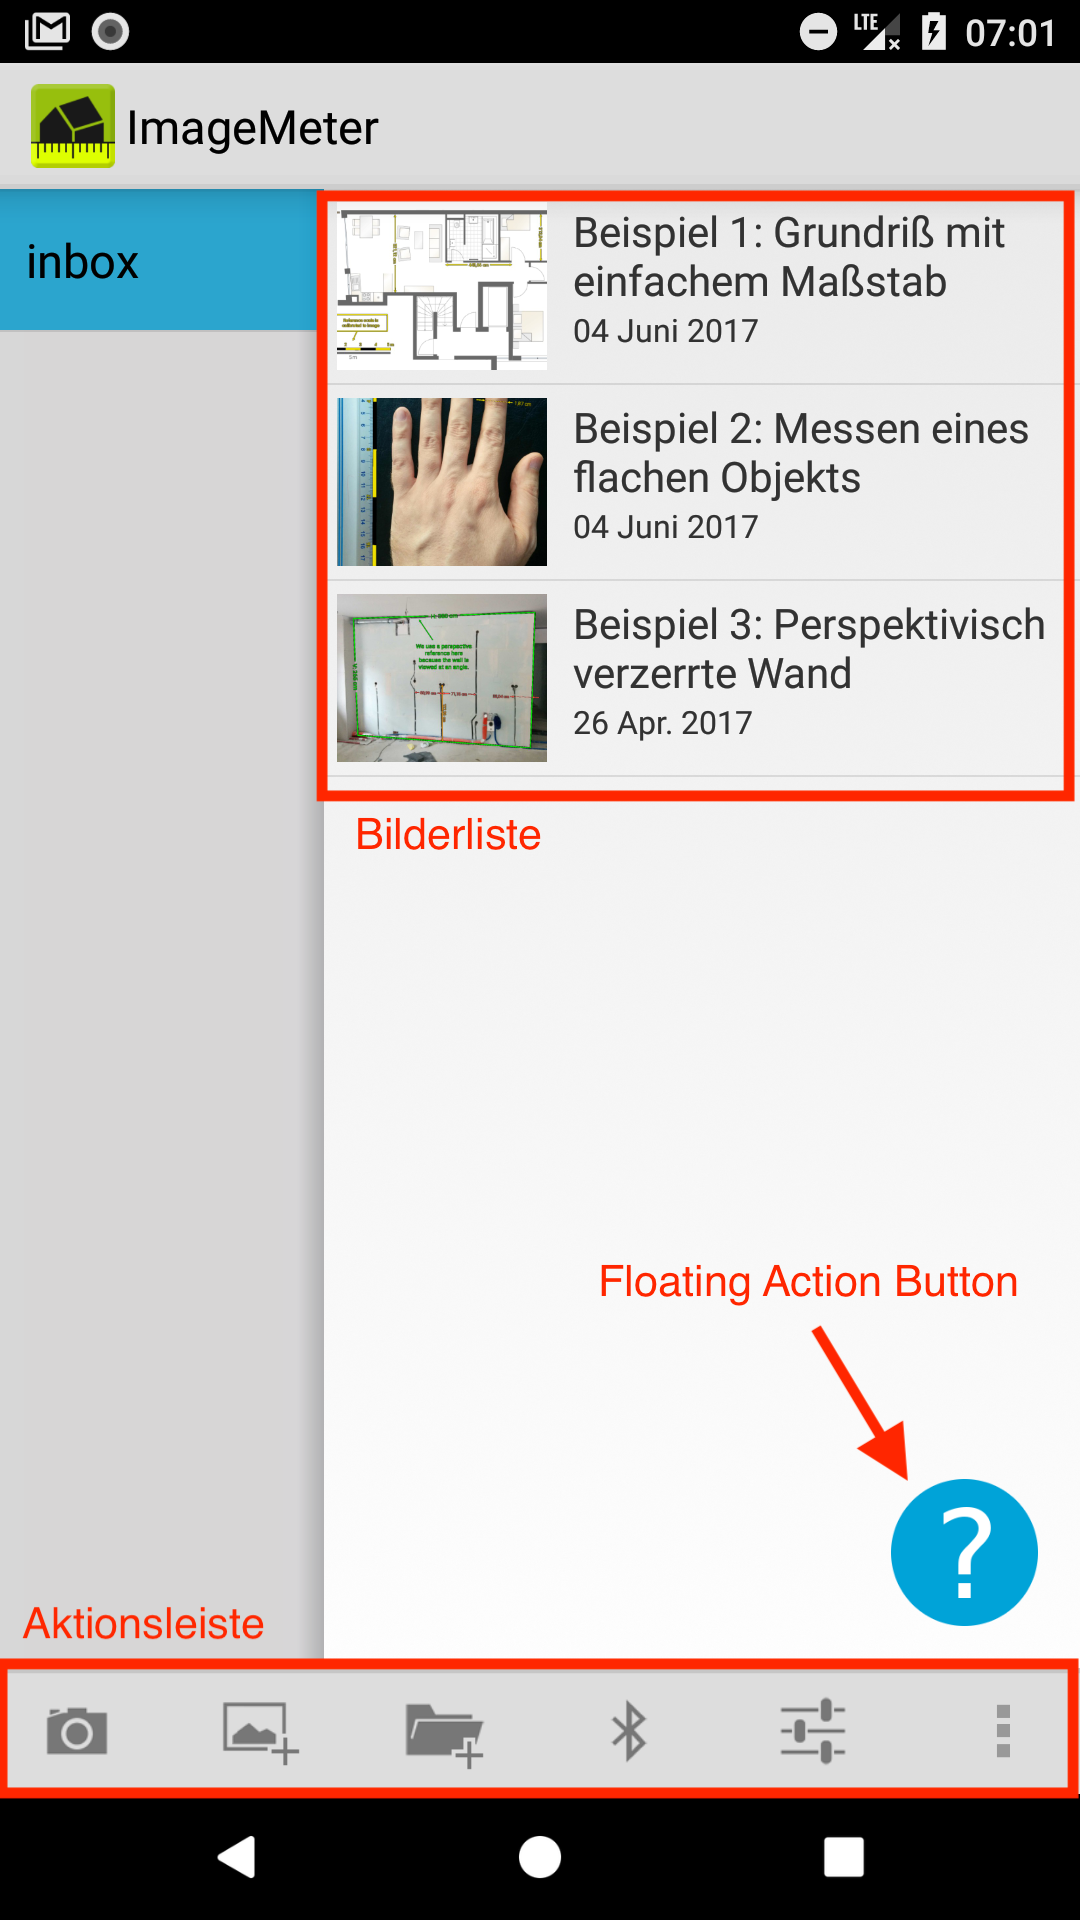
\includegraphics[keepaspectratio, width=\textwidth]{photo_measures/menu}
    \caption{Startbildschirm}
    \label{fig:pmmenu}	
  \end{subfigure}
  \begin{subfigure}[t]{0.4\textwidth}
    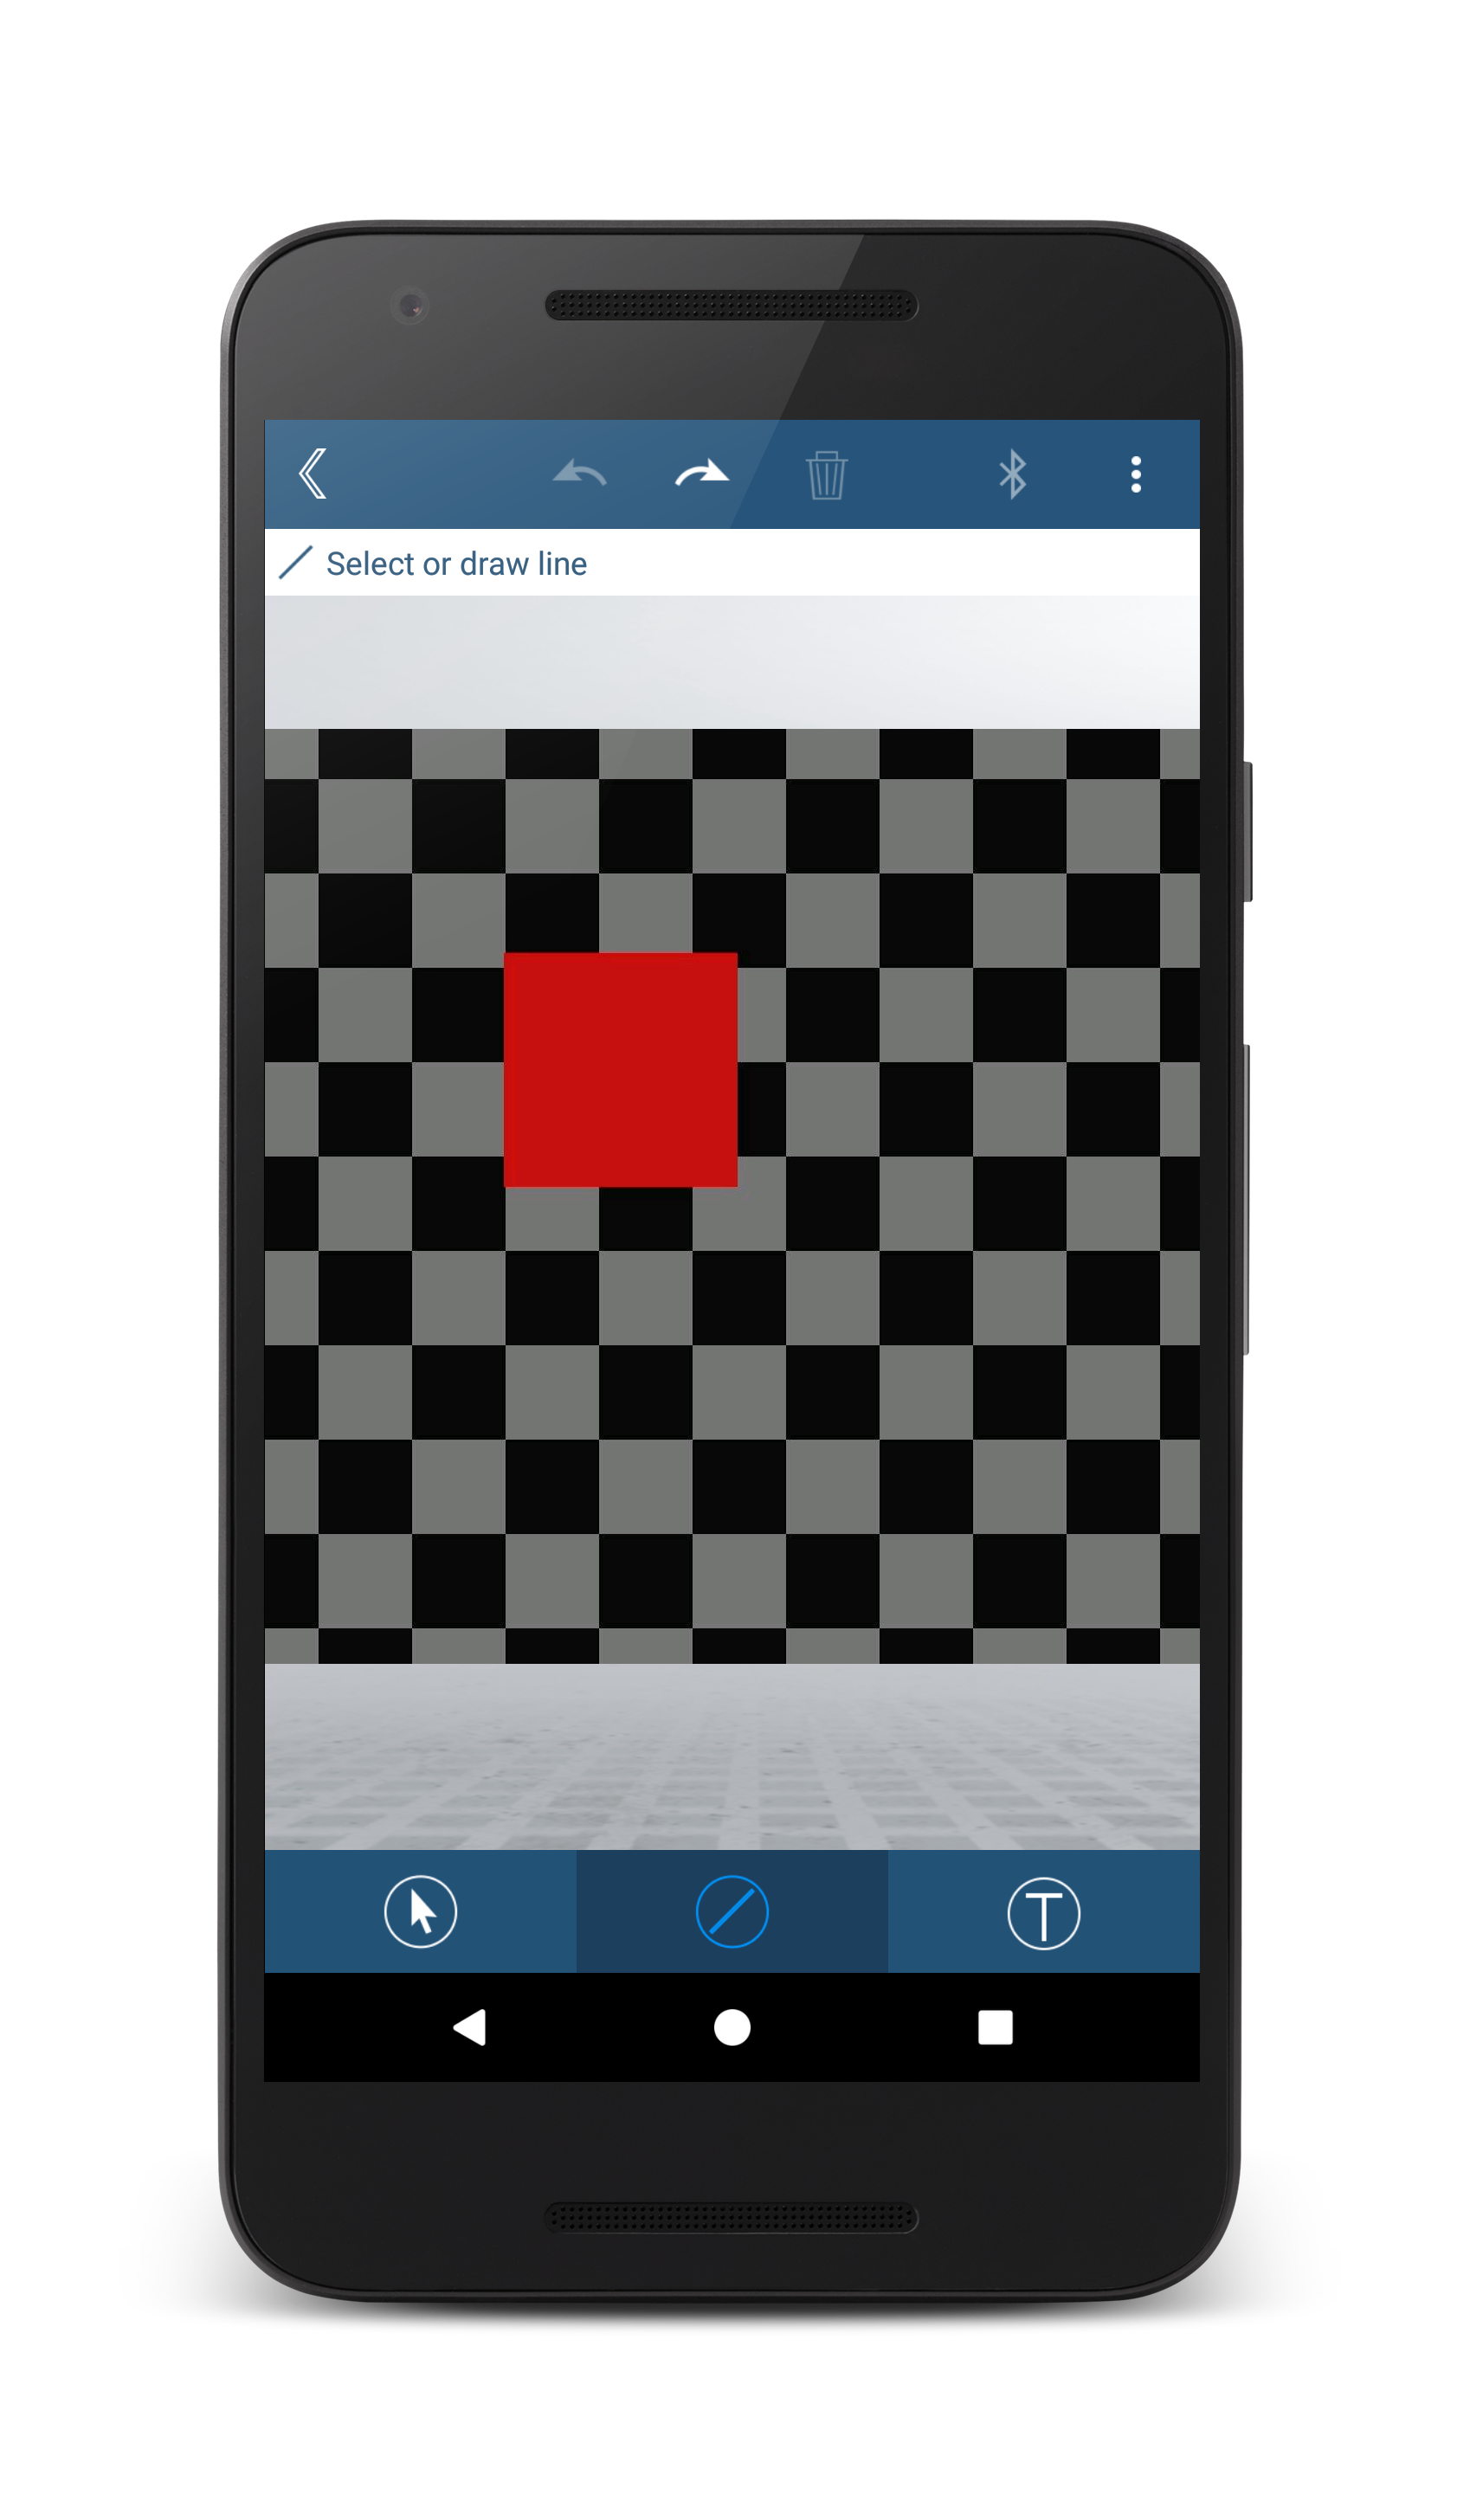
\includegraphics[keepaspectratio, width=\textwidth]{photo_measures/help}
    \caption{Hilfe-Overlay beim initialen Start der Aufmaß-Funktion} 
    \label{fig:pmhelp}	
  \end{subfigure}
  \caption{\pm{} beim Start der App und in der Aufmaß-Funktion}
\end{figure}

\noindent
Durch einen Klick auf das beschriebene Plus-Symbol öffnet sich ein Dialog, der den Benutzer auffordert, ein Bild auszuwählen.
Hierzu kann der Benutzer das Bild direkt aus der Galerie importieren, oder ein Neues mit der Kamera aufnehmen. \\
Anschließend wechselt die App in eine andere Benutzeroberfläche, in der das ausgewählte Bild und eine Statusleiste am unteren Rand des Bildschirms zu sehen sind (\autoref{fig:pmhelp}).
Wenn der Benutzer diese Oberfläche zum ersten Mal öffnet, zeigt die App außerdem ein Hilfe-Overlay, welches dem Benutzer darüber informiert, wie Formen in das Bild eingezeichnet werden können.  \\

Zudem werden nur die Funktionen, die zum jeweiligen Systemzustand ausführbar sind (z.B. Farbe ändern nur wenn Form ausgewählt), in der Statusleiste am unteren Bildschirmrand angezeigt.
Die Statusleiste bietet, wenn keine Form ausgewählt ist, die Möglichkeit zwischen drei verschienden Formen (Linie, Winkel, Freitext) zu wählen, die gewünschte Größe einzustellen, oder das Bild schrittweise um 90 Grad im Uhrzeigersinn zu drehen.
Wenn eine Form ausgewählt ist, kann diese über die Statusleite im Nachhinein beschriftet, gefärbt oder gelöscht werden. \\

Auch in dieser App lassen sich gespeicherte Bilder zu einem späteren Zeitpunkt weiter bearbeiten.
Außerdem können mehrere Bilder gleichzeitig zusammen in einer \emph{PDF} oder als jeweils einzelnes Bild geteilt werden.

\subsubsection{Evaluation}\label{subsec:pmeva}

Hilfe und Dokumentation (Nielsen~\autoref{itm:N10}) werden in dieser App in Form eines Hilfe-Overlays, welches beim intialen Start angezeigt wird, und im Nachhinein über einen dedizierten Button erreichbar ist, bereit gestellt (siehe \autoref{fig:pmhelp}). \\

Des Weiteren sind Aktionen nur dann verfügbar bzw. auswählbar, wenn diese im aktuellen Systemzustand legal sind.
Dies vermeidet einerseits Situationen in denen Fehler entstehen können, andererseits gibt dies dem Benutzer eine angemessene und verständliche Rückmeldung über den derzeitigen Systemzustand der App (Nielsen~\autoref{itm:N1} \& \autoref{itm:N5}). \\

\begin{wrapfigure}{R}{0.4\textwidth}
  \centering
  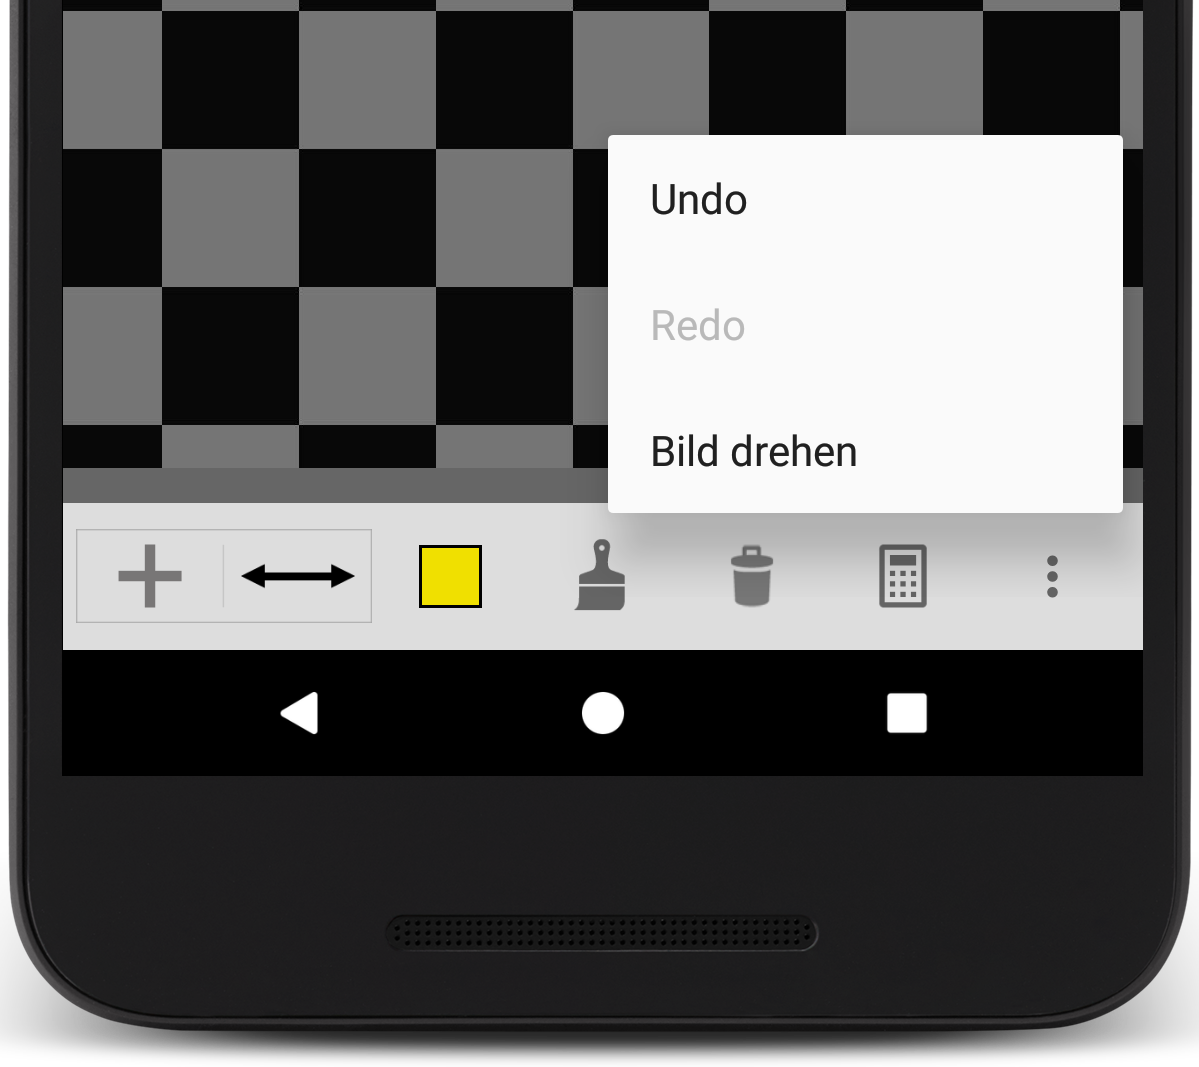
\includegraphics[keepaspectratio, height=0.4\textheight]{photo_measures/bar}
  \caption{Statusleiste im Zeichen-Modus bei Ausrichtung der App im Querformat}
  \label{fig:pmbar}
\end{wrapfigure}

\noindent
Die App bedient sich einer Reihe universell bekannter Icons, sodass intuitiv erkennbar seien sollte, welche Aktion sich hinter welchem Button verbirgt.
Wird ein Icon dennoch nicht erkannt, so stehen zusätzlich die Aktionen in Textform unter diesen (siehe \autoref{fig:pmbar}). \\

Außerdem hat der Nutzer die Möglichkeit, Formen, Größen und Farben im Vornherein beliebig anzupassen.
Dies fördert nicht nur eine flexible Benutzung der App, sondern steigert gleichzeitig die Effizienz, da die App nur einmal zu Beginn der Benutzung wie gewünscht eingestellt werden muss. \autoref{itm:N7} \\

Im Gegensatz dazu steht die fehlende Benutzerkontrolle \autoref{itm:N3} der App.
So ist es dem Benutzer nicht möglich, über einen Undo- bzw. Redo-Button seine Aktionen zu revidieren.
Dies ist gerade bei der Bearbeitung von Bildern, bei der es viele aufeinander aufbauende Aktionen des Benutzers gibt, eine entscheidende Funktionalität, welche nicht nur die Gedächtnisbelastung senken, sondern auch den ``Joy of Use'' deutlich steigern kann. \\

Zudem fällt auch in dieser App die fehlerhafte Zoom-Geste auf, welche dazu führt, dass während des Zoom-Vorgangs eine Form auf das Bild gezeichnet wird (Nielsen~\autoref{itm:N16}).
Dies erzwingt nach fast jeder Zoom-Geste einen Lösch-Aktion der unabsichtlich gemalten Form, da es keine Undo- bzw. Redo-Funktion gibt. \\

Ein positiver Aspekt dagegen liegt in der Unterstützung verschiedener Bildschirmausrichtungen, sowie dem adäquaten Umgang mit Unterbrechungen.
So lässt sich das Gerät beliebig drehen, ohne dass Informationen in der App verloren gehen, oder der Benutzer durch eine unerwartete Ausrichtung des Bildes bzw. der Statusleiste verwirrt wird (Nielsen~\autoref{itm:N11} \& \autoref{itm:N15}). \\

Die einfache Handhabung und das Zeichnen von Formen mit einem Finger ermöglichen eine einhändige Benutzung der App und wirken sich damit positiv auf die Benutzererfarhung aus (Nielsen~\autoref{itm:N13} \& \autoref{itm:N17}).
Außerdem stellt auch diese App beim Zeichnen von Formen den vom Zeichenfinger verdeckten Bereich des Bildschirm vergrößert an einer anderen Stelle dar \todo{Bild}.
Dies beugt Fehlern vor und erhöhrt zudem die Nutzungserfahrung, da der Nutzer hierdurch in der Lage ist, Formen bis zu einem gewünschten Punkt zu zeichnen, ohne den Finger vom Bilschirm nehmen zu müssen um zu sehen, bis wohin sich die Form bereits erstreckt.

Auch diese App ermöglicht es weder Bilder aus einer anderen App heraus in diese direkt freizugeben, oder bearbeitete Bilder inklusive der Meta-Daten an eine andere App zu teilen.
Zudem gehen beim Exportiren der annotierten Bilder alle eingetragenen Messwerte in Form von Meta-Daten, die zur Weiterverarbeitung benötigt werden, verloren.

Zusammenfassend kann also festgehalten werden, dass die App \pm{} von \emph{Big Blue Pixel} keine Möglichkeit bietet, Messwerte, die in ein Bild eingetragen wurden, zur Weiterverarbeitung
in der bestehenden Android-App oder in einem nachgeschalteten Dienst wie einer \emph{API} zugänglich zu machen. \\

Die Nielsen-Heurstiken werden größtenteils erfüllt, jedoch wurden auch einzelne Punkte nicht gut umgesetzt.
So führen die fehlerhafte Zoom-Geste, die bei jeder Zoom-Aktion eine Form zeichnet, in Kombination mit der gänzlich fehlenden Undo/Redo-Funktionalität zu einem negativen Nutzungserlebnis der App.
Besonders diese fehlende Benutzkontrolle ist bei der Bearbeitung von Bildern, in der sich das Endergebnis aus einer Vielzahl von kleinen Benutzeraktionen zusammensetzt, als besonders schwerwiegend zu gewichten.
Hierdurch entstehen Fehler, die es durch die Nutzung einer Android-Applikation zu verhindern galt.

